\chapter{Preliminaries}\label{preliminaries}
To get a better understanding of our research, we provide some preliminary information in this section. We will start by introducing the concept of \emph{reinforcement learning} in section \ref{pl-rl}. Following this, we will discuss \emph{state-space dimensionality reduction}, including several methods to do this in section \ref{pl-dimensionality}.
 
\section{Reinforcement learning}\label{pl-rl}
The main theoretical framework we are working in is called \emph{reinforcement learning} (RL). This is a form of \emph{machine learning}: the area of artificial intelligence that is concerned with creating computer programs that can solve problems by learning from data. The two other main forms of machine learning are \emph{supervised learning} and \emph{unsupervised  learning}. The distinct feature of RL is that it learns from feedback through trial and error \cite[p. 2-5]{grokking}.

We will now examine RL more closely and formally, as well as discuss \emph{neural networks} and a specific RL algorithm used in our research called \emph{DDQN}.

 
\subsection{General overview}
As mentioned, RL is the area of artificial intelligence where problems are solved through trial and error using feedback. An example is a robot learning to bring a given package to a given location. The portion of the code responsible for the decision-making, i.e. choosing an action, is called the \emph{agent}. Besides an agent, there is also the \emph{environment}, which entails everything other than the agent. In our package delivery example, this could for instance be the hardware of the robot, the package to be delivered, wind conditions, the road, and any obstacle.

The environment is encoded in a set of variables, where all possible value-combinations of these variables are called the \emph{state-space}. In our example, some of these variables denote the coordinates of the location of the robot, wind speed and direction, and the coordinates for the location where the package needs to be delivered. A single instantiation of the state-space is a \emph{state}. 

To be able to make an informed decision, the agent will need some information with regard to the current state. The information about a state received by the agent, i.e. the variables making up the state-space, is called an \emph{observation}. This observation might be partial; the agent might not receive all information about a state. In our example, the agent might not have any information about an obstacle on the road that it hasn't sensed yet.

Using this information, the agent makes a decision  about which action to take. The total set of possible actions for all states is the \emph{action-space}. A lot of different algorithms exist with regard to decision-making and learning how to make better decisions. In section \ref{pl-dqn} we will discuss the learning algorithm we will use, called \emph{double deep-Q-network}. Depending on the current state and the action taken by the agent, the environment might go to a new, different state. This change is encoded by a \emph{transition function}; given a state and action pair it returns the next state. 

The current mapping in the agent between a given state and a distribution over possible actions is called its \emph{control policy}. The better its policy, the better it is able to solve the problem. To be able to improve its policy, the agent needs information about how well it has been performing. This feedback is given in the form of \emph{rewards}: the environment sends positive or negative rewards to the agent, informing it about how well it has performed. In our package delivery example, the robot might get a $+1$ reward whenever it delivers a package.

This results in an interaction cycle between the agent and the environment, depicted in figure \ref{fig:rl_cycle}. It begins with the agent receiving an observation. Then, it chooses an action. This results in the environment transitioning into a new state (possibly the same state as before having taken the action). After this, the environment sends a new observation along with a reward to the agent, and the agent chooses a new action. This interaction stops once the problem has been solved, or when some other constraint has been violated (like a time limit, or the robot getting into an unwanted state like the robot crashing into an object). When the cycle stops, we have finished an \emph{episode}. After this, the environment can be reset to start a new episode. To get to a well-performing policy, the agent often needs hundreds or thousands of episodes \cite[p. 6-10]{grokking}. 

\begin{figure}[h]
    \centering
    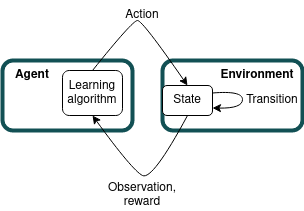
\includegraphics[width=0.45\textwidth]{rl-cycle}
    \caption{The cycle of interaction between the environment and an agent in reinforcement learning.}
    \label{fig:rl_cycle}
\end{figure}

Let us now formally define the reinforcement learning paradigm. RL problems are commonly modeled as \emph{Markov decision processes} (MDPs). 

\begin{definition} A Markov decision process (MDP) is a tuple $(S, A, T, R, S_{\theta})$, with state-space $S$, the action-space $A$, transition  probability function $T$: $S \rightarrow 2^{A \times Distr(S)}$ (thus modeling stochasticity), reward function $R$: $S \times A \times S \rightarrow \mathbb{R}$ and initial states distribution $S_{\theta}$. $T$ also describes the probability distribution for transitions, $p(s'|s,a)$: the probability of transitioning to state $s'$ given state-action pair $(s, a)$ \cite[p. 45-62]{grokking}.
\end{definition}

A graphical example of an MDP can be seen in figure \ref{fig:mdp}.

\begin{figure}[h]
    \centering
    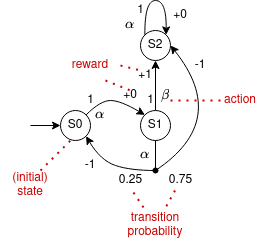
\includegraphics[width=0.5\textwidth]{MDP}
    \caption{Example of a Markov decision process (MDP).}
    \label{fig:mdp}
\end{figure}

The reward function models the expected reward for a transition; given a transition consisting of a state, action, and next state, it returns the expected reward.

The reward function is defined as function $r$:
\begin{equation}
	\label{reward}
	r(s, a, s') = \mathds{E}[R_{t} | S_{t-1} = s, A_{t-1} = a, S_{t} = s']
\end{equation}
where $t$ is the timestep and $R_{t} \in R \subset \mathbb{R}$ \cite[p. 54]{grokking}.

To get to its best possible policy, an agent tries to maximize its total sum of expected rewards. This is also known as the \emph{return} $G$: 
\begin{equation}
G_t = R_{t+1} + \gamma G_{t+1}
\end{equation}
with timestep $t$ and a discount factor $\gamma \in [0,1]$ to set the weight of future rewards \cite[p. 67]{grokking}. 

Often, an agent does not know the underlying MDP to a problem. Therefore, we must use a way without using the underlying MDP to find the optimal policy (i.e. the policy giving the highest expected return). To evaluate any policy ${\pi}$ and be able to compare its performance to other policies, we can use the \emph{Bellman equation}. This tells us what the expected return is when starting at any state $s$, following policy $\pi$. This is known as the \emph{state-value function} (V-function, or $V^{\pi}(s)$).
\begin{equation}
v_\pi (s) = \sum_{a} \pi (a|s) \sum_{s', r} p(s', r|s,a)[r + \gamma v_\pi (s')], \forall s \in S
\end{equation} 

For any state, we look at all possible actions. For each resulting state-action pair, we look at all possible transitions and sum the corresponding reward with the value of the next state weighted by the discount factor $\gamma$. This sum is then weighted by the probability of this transition. The resulting value is summed for all possible transitions of this state-action pair, and we then sum these results for all actions of the given state. This results in the value for this state \cite[p. 73]{grokking}.

Having a method of finding the value of a state, is the first step towards an agent being able to figure out the best possible policy. When an agent tries to improve its policy, it can make use of the \emph{action-value function} (Q-function, or $Q^\pi (s, a)$. This tells us the expectation of returns following policy $\pi$ after having taken action $a$ in state $s$. It is defined as follows:

\begin{equation}
q_\pi (s,a) = \sum_{s', r} p(s', r|s,a)[r + \gamma v_\pi (s')], \forall s \in S, \forall a \in A(s)
\end{equation}
For all possible state-action pairs $(s,a)$, we calculate their value by looking at all their possible transitions, taking the corresponding reward, summing this by the state-value of the next state weighted by the discount factor $\gamma$, and weighing this sum with the probability of this transition happening \cite[p. 74]{grokking}.

An agent is in search of an optimal policy: a policy that has an expected return greater or equal to all other possible policies. Such a policy has the optimal action-value function, known as the $q*$ function: this is the action-value function with the highest value over all possible policies. Therefore, if the agent is able to figure out the $q*$ function, it knows the optimal action for each state and thus the optimal policy. 

Approximating this $q*$ is the approach for most current state-of-the-art learning algorithms, including the one used in this research: double deep-Q-network (DDQN). These types of agents are called \emph{value-based RL agents}. Furthermore, learning algorithms might be \emph{model-based} or \emph{model-free}. In model-based algorithms, the RL agent tries to construct and use an MDP model of the environment. In  model-free agents, the agent directly learns a control policy. The latter is used in our research, using DDQN.

We will explain how DDQN is able to approximate the $q*$ function in section \ref{pl-dqn}. However, to understand DDQN, we will first need to introduce \emph{neural networks}. This is because in order to approximate the $q*$ function, an agent will need to keep track of the action-value for all state-action pairs. Storing these values in a table is not scalable: for problems with large (or continuous) state-spaces and large action-spaces, the table would become way too large to be able to work with. Therefore, we need a way to approximate this table, which is what neural networks are used for. We will now first explore neural networks, before explaining DDQN.

\subsection{Artificial neural networks}\label{pl-nn}
The use of artificial neural networks (ANN) in reinforcement learning, is known as \emph{deep RL} \cite[p. 5]{grokking}. ANNs are a way of being able to use RL in problems with large state-spaces and large action-spaces. This is because ANNs are able to approximate both linear and non-linear functions in an efficient way\cite[p. 165-166]{nn}. Therefore, they can be used to approximate the $q*$ function, instead of using an action-value table to know the $q*$ function. We will now shortly examine ANNs, using \cite[p. 164-366]{nn}.

ANNs consist of artificial neurons: a mathematical function that sums its input which is used to produce an output. These neurons are grouped into different layers, consisting of any number of neurons. Firstly, there is the input layer. In the case of RL, its input is most often the variables making up an observation. Secondly, there is the output layer, creating the output of the network. In between these two layers there usually are other layers. These are known as the hidden layers. 

To produce an output, a neuron sums its input. Each input of a neuron has its own weight: a variable setting its importance. The network learns to produce better output by changing these weights. After summing the weighted inputs and adding a bias, the result is passed through an (often nonlinear) activation function. This produces the output of the neuron. 

Different types of neural networks exist. One important difference here is the connections between neurons. The simplest form is a \emph{feedforward} neural network. Here, each neuron is only connected to neurons of the next layer, meaning there are no cycles. They are often fully connected: a neuron passes its output to each neuron of the next layer. An example of a fully connected feedforward neural network can be seen in figure \ref{fig:nn}.

Another important type of neural network is a \emph{convolutional neural network} (CNN). This is a network that is useful for grid-like data, like image data. It is well suited for applications like image recognition. Such a network makes use of at least one convolutional layer. A convolutional layer consists of multiple filters (or: kernels): a set of trainable parameters. Each kernel convolves across the input to produce a feature map (or: activation map). Since each kernel has different parameters, each feature map will highlight different features of the input. These feature maps are then stacked to produce the output of the convolutional layer. This process is shown in figure \ref{fig:cnn}, where a convolutional layer with a single filter is shown. Adding filters would mean that those filters would convolve in the same way over the same input, creating multiple feature maps that are stacked to produce its output.

\begin{figure}[h]
    \centering
    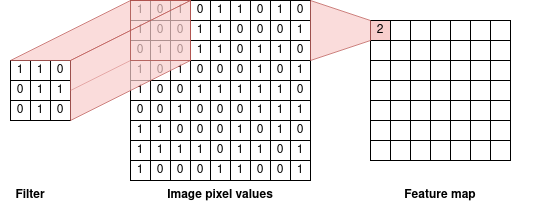
\includegraphics[width=0.75\textwidth]{CNN}
    \caption{A convolutional layer with a single filter. The filter convolves across the input image to produce one feature map. Adding more filters would result in a stack of feature maps (one per filter).}
    \label{fig:cnn}
\end{figure}

To improve the given output, a network can update its weights. For this, it needs a loss function that computes how incorrect the given output was. To calculate how much each weight needs to be changed, backpropagation is used. This computes the gradient for each weight with respect to the loss function. This way, the loss can be minimized and therefore the output optimized.

\begin{figure}[h]
    \centering
    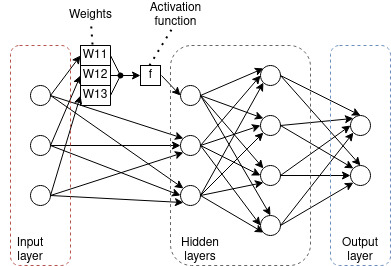
\includegraphics[width=0.5\textwidth]{nn}
    \caption{Example of a fully connected feedforward artificial neural network. For one node, example weights and activation function are shown.}
    \label{fig:nn}
\end{figure}

For more details on artificial neural networks, we refer to \cite{nn}. ANNs are a central part of the learning algorithm used in this thesis: double deep-Q-network, which we will now examine.

\subsection{Double deep-q-network}\label{pl-dqn}
Before going into the learning algorithm DDQN, it is useful to start by looking at other algorithms preceding DDQN. Firstly we will look at \emph{Q-learning} and \emph{deep-Q-learning} (DQN). 

The RL approach taken in Q-learning is arguably the most used in RL \cite{qlearning}. It uses a table, the Q-table, to keep track of the Q-function determining the agent's policy. This Q-table is updated with new information gathered by the agent, to ultimately find an optimal policy by approximating $Q*$.

This is done through a cycle of interactions of the agent with the environment. The agent starts by getting an observation and choosing an action. The environment moves to a new state and the agent receives a new observation and a reward for the current transition. Then the Q-table is updated and the cycle starts over until we reach the end of our episode. Depending on the problem, the agent will need hundreds or thousands of episodes to get the Q-table to approximate the $Q*$ function.

When choosing an action, exploitation needs to be balanced with exploration. The agent needs to explore different actions in the same state to find out all possible outcomes and explore as many states as possible. Simultaneously, the agent will only start performing well once it starts exploiting the updated Q-table. To do this, an \emph{$\epsilon$-greedy strategy} is used. Each time an action must be taken, the agent gets a random number between $0$ and $1$. Whenever this is lower than or equal to the $\epsilon$ value, a random action is taken, otherwise, it chooses an action greedily based on the Q-table. In this strategy, $\epsilon$ is usually decayed over time, to slowly put more emphasis on exploitation.

To update the Q-table after a transition, the old Q-value is added to the new information gotten from this transition, known as the \emph{temporal difference}. The temporal difference is first weighted by a hyperparameter called the \emph{learning rate}. This temporal difference is the difference between the current estimate in the Q-table and the \emph{TD-target}, which is the Q-value we are now moving towards. Thus, it represents the error between the current Q-value and the new estimate and is therefore known as the \emph{TD-error}.

\begin{equation}
Q(s_t,a_t) \leftarrow Q(s_t,a_t) + \alpha \cdot (r_t + \gamma \cdot \max _{a} Q(s_{t+1},a) - Q(s_t,a_t))
\end{equation}

In this equation, $r_t$ is the reward for this transition, $\alpha$ the learning rate and $\gamma$ the discount factor. The TD-target is calculated by adding the reward to the maximum Q-value of the next state weighted by the discount factor. Subtracting the old Q-value from the TD-target gives the TD-error. 

As mentioned in section \ref{pl-rl}, the use of a Q-table is not scalable. Therefore, new algorithms were introduced that use neural networks. One such algorithm is DQN. DQN was first introduced in 2015 by V. Mnih, K. Kavukcuoglu, and D. Silver, and was the first algorithm to apply RL to high-dimensional data while getting human-level scores for Atari-games \cite{dqn}.

Instead of computing Q-values directly using a Q-table, DQN \emph{approximates} the Q-function using neural networks. Such a network takes as input a state observation and produces as output the Q-value for all possible actions in this state. To act greedily, the agent must simply pick the action with the highest value in the output of the network.

To get the Q-values for a state, we pass the state to its policy network. This is the network representing the policy of the agent. To be able to compute the TD-error, we also pass the next state to a network, to get the max Q-value of the next state. However, we use a second network for this. If we were to use the same network, the target would change every time the policy network is updated, thereby having it chase its own tail. Having a second network, the target network, allows us to freeze targets for a certain number of steps (a hyperparameter), before updating the target network to equal the policy network.

Additionally, we don't train the policy network with every step but use a hyperparameter to set how often we train the network. Thus, we must store \emph{experiences}: tuples containing information about a transition, including the initial state, next state, reward, and whether we ended in a terminal state. When training the network, we train it on batches of these experiences, known as \emph{replay memory}. 

Thus, when training the policy network, we pass batches of the next states to the policy network to get their maximum Q-values. The corresponding rewards are added to calculate the TD-target. Then the initial states are passed to the policy network to get their Q-values. These values are then used to calculate the TD-error which is used to calculate the loss using the loss-function. Then the policy network is updated by backpropagating the loss.

Now we can look at the algorithm used in this thesis: double-DQN (DDQN). An overview of how a DDQN agent works is given in figure \ref{fig:ddqn}. DDQN is very similar to DQN. The difference is in how the policy network is trained \cite{ddqn}. In DQN we are taking the maximum of all Q-values. Since these values are estimates that differ from their true value, DQN tends to overestimate the highest Q-value. Doing this often will lead to divergence \cite[p. 293-297]{grokking}. Implicitly we are using the target network for two things: to get the action with the highest value, and what its value is. To solve the problem of overestimating Q-values, DDQN separates these two concerns: we use the policy network to get the action with the highest Q-value and then use the target network to get this action's Q-value. This way, the target network cross-validates the estimates of the policy network.

\begin{figure}[h]
    \centering
    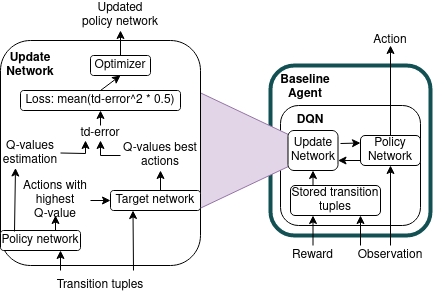
\includegraphics[width=0.6\textwidth]{DDQN}
    \caption{An overview of how a DDQN RL agent works.}
    \label{fig:ddqn}
\end{figure}

The pseudocode for DDQN is given in algorithm \ref{alg:ddqn}. This shows its training step for optimizing the policy network. This method is called within the interaction between agent and environment as explained in section \ref{pl-rl}. In short, the agent will receive an observation from the environment and the agent will, in our case, use a {$\epsilon$}-greedy strategy to choose an action. Then, the environment transitions and gives a new observation to the agent. Hyperparameters are used to set the number of such steps in between training the policy network, and to set the number of steps between updating the target network.

\begin{algorithm}
\caption{DDQN training step \cite[p.299]{grokking}.}
\label{alg:ddqn}
\begin{algorithmic}[1]
\State Sample $experiences$ from replay buffer
\State $states$, $actions$, $rewards$, $next\_states$, $terminals$ $\gets$ $experiences$
\State $indices\_a\_q\_sp$ $\gets$ $\argmax_a policy\_ network(next\_states)$
\State $q\_sp$ $\gets$ $target\_network(next\_states)$
\State $max\_a\_q\_sp$ $\gets$ $q\_sp[indices\_a\_q\_sp]$
\State $max\_a\_q\_sp$ $\gets$ $max\_a\_q\_sp$ $\cdot$ $(1-terminals)$ \Comment{where in $terminals$ True equals $1$, \null $\qquad\qquad\qquad\quad\qquad\qquad\qquad\qquad\qquad\enskip\qquad\qquad\qquad\qquad\qquad\qquad$ False equals $0$.}
\State $target\_q\_sa$ $\gets$ $rewards + \gamma \cdot max\_a\_q\_sp$
\State $q\_sa \gets policy\_network(states, actions)$
\State $td\_error \gets q\_sa - target\_q\_sa$
\State $loss \gets mean(td\_error^2 \cdot 0.5)$
\State Optimize $policy\_network$ with backpropagation using $loss$
\end{algorithmic}
\end{algorithm}

\section{State-space dimensionality reduction}\label{pl-dimensionality}
In RL, states and observations are determined by variables, as mentioned in section \ref{pl-rl}. A single state is simply a single instantiation of these variables. All possible values of these variables together form the total state-space. A larger state-space means more computing costs for the agent. This has several reasons. Firstly, the agent needs to explore more states to explore the entire state-space. This in turn means having to gather larger datasets containing observations, which can be impractical \cite{AE_2019}. Secondly, for an agent to be able to form a decent policy, the policy network (and target network in the case of DDQN) needs to be of an appropriate size. When it is too small for a certain state-space, it will not be able to approximate the Q-function well enough. Therefore, in general, the larger the state-space, the larger the policy network has to be. Training and using a larger network takes more computing costs, since we are dealing with more trainable variables (i.e. the weights of a neural network) \cite{AE_2019}. This is especially true for CNNs, which are commonly used in RL when dealing with image data \cite{CNN_computation}. Lastly, higher dimensional data may include more noise, which can prevent an agent from finding an optimal policy \cite{AE_2016}. Thus, having a smaller state-space results in less computationally expensive agents; decisions can be made quicker (since a forward pass through the network will be slightly faster) and the agent is able to faster converge to a good policy. 

The size of the state-space is problem and environment specific. Generally, more complex problems and environments come with larger state-spaces. A way of dealing with large state-spaces is needed for RL to be scalable. One such way is to make the state-space of a specific problem smaller while retaining enough information for the agent to get to a good policy. This problem of reducing the dimensionality of the state-space while keeping the necessary information for an agent to train on is known as \emph{state-space dimensionality reduction}.  %TODO citation voor tweede zin?

Several methods for state-space dimensionality reduction exist. We will discuss and use three of them in this research: \emph{principal component analysis}, \emph{autoencoder}, and \emph{deepmdp}. We will now discuss these methods in detail. %TODO deepmdp gebruikt?
\subsection{Principal Component Analysis}\label{pl-pca}
The first method for state-space dimensionality reduction we will discuss is \emph{principal component analysis} (PCA) \cite{pca}. 

The general idea of using PCA to reduce the dimensionality of the latent space, is to apply PCA to a state observation of the agent immediately after receiving it from the environment. Applying PCA will project the observation data to a lower dimensional space. This lower dimensional observation will then be the observation the agent will use. Thus, the dimension PCA projects to determines the new state-space dimensionality \cite{mario}.

The first important mathematical concept behind PCA is the \emph{covariance matrix}. This computes the covariance between each variable-pair, thereby computing their correlation. To compute the covariance matrix, we first subtract the mean of each column in the original data matrix from every value in that column. Then, depending on whether variance between features corresponds to the importance of that feature, we may standardize the data by dividing each value by the standard deviation of its column. This results in matrix $X$. To compute its covariance matrix, we simply transpose $X$ and multiply it with $X$ giving matrix $X^TX$.

The other two important mathematical concepts behind PCA are \emph{eigenvectors} and \emph{eigenvalues}. An eigenvector $v$ of a matrix $X$ is a vector such that multiplying it with $X$ results in a variable number of vectors $v$:

\begin{equation}
\label{eigenvectors}
X \cdot v = \lambda \cdot v
\end{equation}

The number of vectors $v$ that we end up with, i.e. $\lambda$ in equation \ref{eigenvectors}, denotes how much we are scaling the eigenvector and is called the \emph{eigenvalue} of that eigenvector. The number of eigenvectors that a matrix has, is at most $min(\#rows, \#columns)$. 

For PCA, we calculate the eigenvectors and eigenvalues of the covariance matrix $X^TX$. These eigenvectors, called \emph{principal components}, represent the axis of the original matrix $X$ with the highest variance, i.e. capturing the most information. Together, all principal components capture the entire original data. However, the higher the eigenvalue of a principal component is, the higher its variance is and thus the more information it captures. Therefore, we sort the eigenvectors based on their eigenvalue; thus the first principal component captures the most information of all principal components. We can then take the first $x$ number of principal components to project the original data onto. Taking for instance $10$ principal components of the original data that contained $15$ features, means we project the original data onto a $10$-dimensional space.

To use PCA for state-dimensionality reduction, we simply apply PCA to state observations that the agent receives from the environment. After applying PCA, the observation is projected to a lower dimensional space (depending on the number of principal components we take). This lower dimensional observation is then further used by the agent, thus training the agent on a lower dimensional state-space.

\subsection{Autoencoder}\label{pl-ae}
Another way of projecting data onto a lower dimensional space, is using an \emph{autoencoder}\cite{AE_general}. An autoencoder is a neural network consisting of two parts: an encoder network and a decoder network. The encoder projects the given input data onto a lower dimensional space, also called the \emph{latent space}. The output of the encoder, called the \emph{latent representation}, is used as input for the decoder. This decoder tries to reconstruct the original input from the latent representation as close as possible. The autoencoder architecture is shown in figure \ref{fig:AE_architecture}.

\begin{figure}[h]
    \centering
    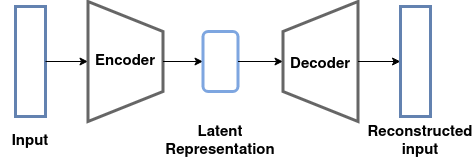
\includegraphics[width=0.75\textwidth]{AE_architecture}
    \caption{The architecture of an autoencoder.}
    \label{fig:AE_architecture}
\end{figure}

Formally, an autoencoder can be defined by the two functions it learns: 
\begin{equation}
  \label{enc}
  \phi :{\mathbb{R}^n}\rightarrow {\mathbb{R}^m}
\end{equation}
\begin{equation}
  \label{dec}
  \psi :{\mathbb{R}^m}\rightarrow {\mathbb{R}^n}
\end{equation}
\begin{equation}
  \label{encdec}
  \phi ,\psi ={\underset {\phi ,\psi }{\operatorname {arg\,min} }}\,{\Delta}(x, \psi \circ \phi (x))
\end{equation}
Equation~\eqref{enc} defines the encoder and equation~\eqref{dec} the decoder, both satisfying~\eqref{encdec} where $\Delta$ is the reconstruction loss function for input x. The closer the output of the autoencoder approximates the original input, the lower the loss.

A fundamental difference with using PCA, is the type of functions that can be approximated for lowering the dimensionality. Since an autoencoder uses neural networks, it can approximate nonlinear functions, as mentioned in section \ref{pl-nn}. This is in contrast with PCA, which can only approximate linear functions. Because of this, an autoencoder can learn more powerful generalizations which leads to lower information loss\cite{AE_general}.

To use an autoencoder for state-space dimensionality reduction, we again (as with PCA) use as input an observation the agent got from the environment. We can train the autoencoder using both the encoder and the decoder to calculate the loss. This training is agnostic to the RL problem. When used in RL, only the encoder is used. The encoder will project the observation input to the dimensionality of the latent space. 

\subsection{DeepMDP}\label{pl-deepmdp}
The last method for state-space dimensionality reduction is a \emph{DeepMDP} \cite{deepmdp}. In contrast with the previous methods, the DeepMDP is a partial RL agent: training the dimensionality reduction goes hand in hand with training the RL agent.

\begin{figure}[h]
    \centering
    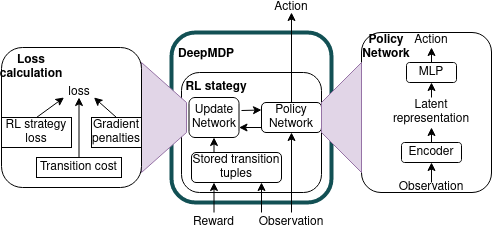
\includegraphics[width=0.75\textwidth]{DeepMDP}
    \caption{An overview of how a DeepMDP agent works.}
    \label{fig:deepmdp_agent}
\end{figure}

This is done through several steps that alter the way the loss for the policy network is calculated. Firstly, there is an encoder neural network that projects the original data to a lower dimensional space, similar to the encoder of the autoencoder. However, in contrast with the autoencoder, this encoder is trained together with the network representing the Q-function using the same optimizer (and thus the same loss). This can be seen in figure \ref{fig:deepmdp_agent}, specifically the \textit{policy network} part. Like a normal value-based RL agent, it trains its policy network using stored transition tuples. Differently from value-based strategies, its policy network now also contains an encoder. An observation first goes through the encoder, lowering the state-space dimensionality, before going into the network representing the Q-function (the \textit{MLP} in figure \ref{fig:deepmdp_agent}). The presence of the encoder will not only project the data to a lower dimensional space but will also influence the loss calculation for the entire policy network since the encoder is trained simultaneously with the network representing the Q-function. 

The loss calculation is also altered in a second way, which in figure \ref{fig:deepmdp_agent} can be seen in the \textit{Update policy network} part. The DeepMDP makes use of an auxiliary objective to calculate the loss, using another neural network: the transition cost network. This network calculates the cost for predicted transitions. For a given latent state (given by the encoder), it calculates the cost for all possible transitions to a next latent state. This means that its output has dimensions $action space \times latent space$. The action space here represents the actions that can be taken in the current latent state, while the latent space represents the next (predicted) latent observation.

Again this network is a part of the agent's network. Consequently, the agent's network consists of three parts: an encoder part, a policy part, and a transition loss part, all trained on the same loss using a single optimizer.

Lastly, a Lipschitz-constrained Wasserstein metric is used. The Wasserstein metric corresponds to the minimum cost of transforming one distribution into another; thus it calculates the cost of moving a particle from a point in one distribution to a point in the other \cite{deepmdp}. The Lipschitz constraint sets a bound to the degree to which a (value) function can change its values. This is implemented by calculating a gradient penalty on all three parts of the network separately (i.e. the Q-function, the encoder, and the transition cost network), as done in \cite{wgan}.

Consequently, the loss calculation is a weighted sum of three parts: the loss calculation of the RL strategy, the transition cost given by the transition cost network, and the gradient penalties for the Q-function network, the encoder network, and the transition cost network.
